% !TEX program = pdflatex
% Drafted from prior personal/camp records. No assigned November 10 math reading used.
\documentclass[11pt,letterpaper]{article}
% Shared visual system adapted from the EDE477 Social Studies Experience Reflection.
\usepackage[margin=0.6in]{geometry}
\usepackage[T1]{fontenc}
\usepackage[utf8]{inputenc}
\usepackage{lmodern}
\usepackage{array}
\usepackage{graphicx}
\usepackage{fancyhdr}
\usepackage{hyperref}
\usepackage{parskip}
\usepackage{ragged2e}
\usepackage{setspace}
\usepackage{needspace}
\usepackage{microtype}
\usepackage[table]{xcolor}
\definecolor{PrimaryRed}{HTML}{8B1E1E}
\definecolor{DeepNavy}{HTML}{15324A}
\definecolor{SoftBlue}{HTML}{DDEEFF}
\hypersetup{colorlinks=true,linkcolor=DeepNavy,urlcolor=DeepNavy,
  pdftitle={Mathematics Experience Reflection},
  pdfauthor={Piter Zacari Garcia Bautista},
  pdfsubject={EDE477 Pre-Reading Reflective Journal},
  pdfkeywords={mathematics, reasoning, camp teaching, evidence, access, identity}}
\setlength{\parindent}{0pt}
\setlength{\parskip}{0.55em}
\setstretch{1.16}
\newcommand{\reviewsection}[1]{%
  \par\Needspace{4\baselineskip}\addvspace{0.10in}%
  \noindent{\large\bfseries\color{PrimaryRed}#1}\par
  \vspace{0.025in}%
}
\newcommand{\bodyformat}{%
  \newgeometry{left=0.75in,right=0.75in,top=0.7in,bottom=0.7in,headheight=14pt,headsep=0.18in,footskip=0.28in}%
  \hypersetup{pageanchor=true}%
  \pagenumbering{arabic}%
  \pagestyle{fancy}\fancyhf{}%
  \lhead{\small Piter Garcia}%
  \rhead{\small EDE477 --- Mathematics Experience Reflection}%
  \cfoot{\small\thepage}%
  \renewcommand{\headrulewidth}{0.4pt}%
}
\widowpenalty=10000
\clubpenalty=10000
\raggedbottom

\begin{document}
\hypersetup{pageanchor=false}
\begin{titlepage}
\thispagestyle{empty}
\begin{center}
{\large University of Rochester\\}
{\normalsize Warner School of Education\\[0.15in]}
{\color{PrimaryRed}\rule{\textwidth}{1.4pt}}\\[0.12in]
{\Huge\bfseries Mathematics Experience\\[0.07in]Reflection}\\[0.14in]
{\huge Counting, Measuring, and Meaning}\\[0.16in]
{\Large EDE477 --- Pre-Reading Reflective Journal}\\[0.12in]
\end{center}
\vfill
\begin{center}
{\large\bfseries\color{DeepNavy}Invisible Invaders \enspace | \enspace EDU486}\par
\vspace{0.14in}
\begin{minipage}[t]{0.33\textwidth}
\centering
{\small\bfseries SAMPLE AND LABEL}\par\vspace{0.07in}
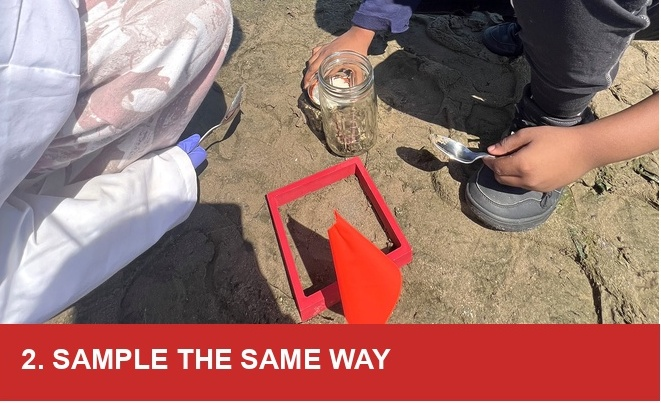
\includegraphics[width=\linewidth,height=1.58in,keepaspectratio]{assets/field-sampling-crop.jpg}
\end{minipage}\hfill
\begin{minipage}[t]{0.33\textwidth}
\centering
{\small\bfseries MEASURE AND CHECK}\par\vspace{0.07in}
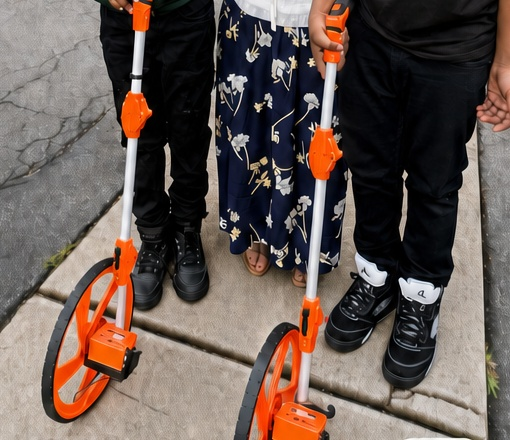
\includegraphics[width=\linewidth,height=1.58in,keepaspectratio]{assets/measuring-wheels-crop.jpg}
\end{minipage}\hfill
\begin{minipage}[t]{0.28\textwidth}
\centering
{\small\bfseries EXPLAIN THE RATE}\par\vspace{0.07in}
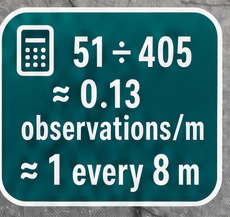
\includegraphics[width=\linewidth,height=1.58in,keepaspectratio]{assets/rough-rate-label.png}
\end{minipage}
\par\vspace{0.12in}
\begin{minipage}{0.96\textwidth}
\footnotesize\RaggedRight
Cropped from our existing \href{https://drive.google.com/file/d/1bKowRD2E0xXEboxJtVNqb9cjKrsoVp8P/view}{Field Friday} and \href{https://drive.google.com/file/d/1Ug-rjUcG6JXRbzDlifEJuga2EnBCmgBi/view}{Litter Meter} recaps (July 2026). Student faces are excluded. These photo-based recap artifacts include designed labels and prior AI-assisted visual work; they are not unedited field records. The rate is a rough summary, not uniform spacing or a complete pollution survey.
\end{minipage}
\end{center}
\vfill
\begin{center}
\colorbox{SoftBlue}{%
\parbox{0.88\textwidth}{%
\centering\small\vspace{0.07in}
\textbf{Doing Mathematics Before the Reading}\\[0.05in]
An answer matters, but so does knowing what was counted,\linebreak
what was measured, and why the comparison makes sense.\par\vspace{0.07in}
}%
}
\end{center}
\vfill
\begin{center}
\renewcommand{\arraystretch}{1.23}
\setlength{\tabcolsep}{5pt}
\begin{tabular}{>{\bfseries\RaggedLeft\arraybackslash}p{1.32in} >{\RaggedRight\arraybackslash}p{5.08in}}
Student & Piter Zacari Garcia Bautista \\
Assignment & \textit{\small Mathematics Experience Reflection} \\
Course & EDE477 --- Teaching and Learning in the Content Areas \\
Module Date & November 10, 2026 \\
Experience Base & \textit{\small EDU486 Invisible Invaders fieldwork, Litter Meter investigation, journals and recap artifacts; TeachingPlacement as a supporting connection} \\
Reading Boundary & \textit{\small No assigned November 10 mathematics reading was consulted in preparing this draft} \\
\end{tabular}
\end{center}
\vfill
\begin{center}
\begin{minipage}{0.95\textwidth}
\small
This reflection revisits my own documented learning and teaching before engaging with the mathematics readings. Its central evidence is our camp experience, not a new literature review. ChatGPT assisted with drafting, source checking, and LaTeX formatting from my prior records and directions. Source provenance accompanies the editable project.
\end{minipage}
\end{center}
\end{titlepage}
\bodyformat
\reviewsection{Finding the Mathematics in Invisible Invaders}

My clearest recent experience of teaching mathematics did not happen in a class called math. It happened in EDU486, when Aastha and I developed and taught \textit{Invisible Invaders} with Freedom Scholars. Looking back through our camp journals, photographs, labels, and posters, I see mathematics throughout the work: predicting, counting, measuring, comparing, mapping, and explaining what a result means. To me, doing math is making sense of relationships and being able to justify an answer, not simply producing a number.

As a student, I began school in Spanish in the Dominican Republic and later studied computer science and data science. That path has made me comfortable working with quantities, but it has also made me question the idea that numbers explain themselves. Software can calculate without knowing whether I chose a meaningful comparison. The camp brought that concern into a setting where the mathematics had a visible purpose: helping us investigate a place and communicate what we noticed.

On Field Friday at Charlotte Beach, learners predicted and counted prepared model pieces, used magnification, and collected sand at flagged locations. Our group and location labels mattered because we needed to know which sample we were examining. The instruction to sample the same way was also mathematical: a comparison depends on what was counted and how it was collected. Looking back, I would make that reasoning more explicit. Before comparing totals, I would ask whether the sampling areas and counting rules were comparable. A larger number alone would not answer that question.

The Litter Meter Mission made this especially clear. We counted visible litter while using measuring wheels. When the distance readings differed, we identified that one wheel had traveled back over a section already measured. The important learning was not just reading the counter; it was connecting its number to the route we intended to measure. That correction helped me see why a mathematically correct calculation can still answer the wrong question when its starting quantities are wrong.

Our camp recap used a recorded count of 51 observations and a rough route of about 400 meters, represented as 405 meters in the visual. Dividing 51 by 405 gives about 0.13 observations per meter, or roughly one observation for every eight meters on average. That does not mean items were evenly spaced eight meters apart. It also does not turn visible litter into chemically confirmed plastic. For me, the value of the calculation was learning what the rate could communicate and where our claim had to stop.

The recap's \textit{count}, \textit{distance}, and \textit{rough rate} labels made that relationship visible beside our photographs. They were not decorations. They helped connect an action, a quantity, and an explanation. I want students to experience mathematics that way: as something they use to investigate and communicate, with room to check and revise rather than hide a mistake.

\newpage
\reviewsection{Teaching for Reasoning, Access, and Belonging}

Invisible Invaders also changed what I pay attention to as a teacher. Our camp reflections document participation through measuring, counting, drawing, recording, pointing, explaining, using tools, and working with a partner. Those contributions gave me more to notice than a finished worksheet. At the same time, an active group does not prove that each learner understands the mathematics. I would still ask each student to explain a quantity or comparison, using a route that lets me see their reasoning.

My Puzzle Plan connects experiences that schools can treat as separate pieces: language, culture, neurodivergence, health, and academic work. My EQUITAS lens asks whose thinking the task makes visible and whose it misses. In math, I do not want fluent English, fast recall, standing through an activity, or polished writing to stand in for understanding. A diagram, home-language explanation, partner rehearsal, or pause can change access without changing the expectation that an explanation must make mathematical sense. I would choose those supports with the learner, not assume a category tells me what someone needs.

The camp was not a perfect model. My final journal records requests for more time to investigate and less rushing. That feedback matters for mathematics: if I move everyone toward the answer too quickly, I may never hear the reasoning I need to understand. I would rather protect time for a useful comparison, an estimate, and a revision than fill the period with steps students can only imitate. Joy also matters to me. Counting, moving, noticing, and questioning together can belong inside demanding work, not merely serve as a reward afterward.

My current business and marketing placement offers a smaller connection. In the paired task I have designed, students distinguish an external factor from its possible effects on a chosen business. With my school-based teacher educator, I could extend that reasoning to a cost or percentage-change problem, making the quantities and assumptions explicit. That is a possible next step, not a mathematics lesson I am claiming to have already taught. The camp remains my strongest example of mathematical thinking embedded in an investigation.

If I were asked to long-term substitute in a math classroom, my raw response would be, ``What grade, and what topic are we working on?'' I would feel nervous and interested. Using math in research does not automatically prepare me to teach every school concept. I would learn the curriculum, look at students' work, and seek guidance while planning questions that reveal how they think. Before the assigned readings, my strongest commitment is this: I want students to leave with more than an answer. I want them to know what it means, explain why it makes sense, and believe that their questions belong in mathematics.

\end{document}
